\chapter{Background}
\label{chap:background}
In this thesis, we will create a robot memory for knowledge sharing and
hybrid reasoning. In order to do so, we first need to introduce
background information. Section~\ref{sec:mobile-robotics} gives an
introduction into the thesis' context of mobile robotics and
reasoning. In Section~\ref{sec:robocup} we introduce the primary
application and evaluation domains, the RoboCup Logistics League
(RCLL) and the RoboCup@Home league. Afterwards, we present the
software context with robot software frameworks in
Section~\ref{sec:robot-software-frameworks} and planners and reasoners in
Section~\ref{sec:planners}.

\section{Mobile Robotics and Reasoning}
\label{sec:mobile-robotics}
A \emph{robot} is a machine capable of automatically carrying out a
  complex series of movements~\cite{robot-dict} and belongs to the
group of \emph{cyber physical systems (CPS)}, which can be defined
as computing elements combined with physical sensing and
  interaction~\cite{chapter-cps}. In contrast to mounted assembly
line robots, we focus in this thesis on \emph{autonomous mobile robots}, thus
robots that are capable of moving in their environment and
are capable of operating without any form of external control
  for extended periods of time~\cite{autonomous-robots}. These robots
interact with their environment to fulfill a specific task they are
designed for. They are \emph{agents}, which utilize a
\emph{sense-think-act cycle}. Sensors perceive the
environment, a computation device decides what to do, and actuators
interact with the environment. How autonomous mobile robots can
act giving its sensing depends on its \emph{agent
  architecture}. Russell and Norvig differentiate the class of simple
\emph{reflex agents} and the class of more advanced
\emph{model-based, goal-based, and learning
  agents}~\cite{aimodern}. Reflex agents can only use the current
sensing to compute how to react and are thus limited in their
capabilities because they can't remember anything from previous
cycles. All other agent architectures have an internal state, which
allows to take the perception history into account and implement more
complex behavior.

\subsection{Robot Memory}
\label{sec:robot-memories}
We define a \emph{robot memory} as a system that memorizes the
internal state of a robot between two or more sense-think-act
cycles. In the case of a model-based agent, it can include a model of
the robots environment to compensate for partial observability of the
domain. A goal-based agent remembers the given goal to achieve in the
environment and a learning agent remembers what was learned from
previous observations~\cite{aimodern}.

Physically, a robot memory can be stored on \emph{volatile} or
\emph{non-volatile} devices that can be read and written. A volatile
device, such as \emph{random-access memory (RAM)}, can only store
information as long as it is powered. Usually, RAM acts as storage
when the internal state of the robot is represented by variables in
the programming languages used to implement the behavior of the
robot.  A non-volatile device, such as a hard disk drive, also keeps
the information when it is not powered. Also a combination of volatile
and non-volatile devices can be used for storage as in this thesis. A
robot memory that is stored on a non-volatile device is called
\emph{persistent}.

\subsection{Knowledge Sharing}
\label{sec:knowledge-sharing}
A robot memory is not necessarily limited to a single robot. In a
\emph{multi-agent system}, a system that is composed of multiple
interacting agents~\cite{multiagentsystems}, the agents can share
their internal state. In this case, a robot memory used for sharing
the state is called
\emph{distributed}. Furthermore, we will call a system composed
of multiple, interacting, autonomous mobile robots a \emph{multi-robot
  system}. Similarly, a robot memory can be shared on a single
robot between multiple agent programs, each implementing a part of
the robot's behavior. The architecture of a multi-agent system can be
\emph{centralized} or \emph{distributed}~\cite{RCLL-Planning}. In the centralized one,
a central unit stores all relevant information and/or decides which
actions each agent should execute. In the distributed one, the
relevant information is stored and synchronized on all agents and/or
each agents makes its own decisions. This introduces the need of
\emph{consistency}, which requires that information stored in a
distributed system has no contradictions.

\subsection{Reasoning}
\label{sec:reasoning}
According to Brachman and Levesque, \emph{reasoning} is the formal
manipulation of symbols representing believed propositions to produce
representations of new ones~\cite{kr-book}. Thus, new knowledge can be
\emph{logically inferred} from other knowledge, by representing the
propositions, which describe what is known or believed, and then
performing reasoning manipulations on it.  A simple example for
logical inference is the following: Based on \emph{Caesar is a robot}
and \emph{All robots should have a memory} it can be inferred that
\emph{Caesar should have a memory}.  The field of \emph{knowledge
  representation} deals with the question how propositions like these
can be represented in logic formalisms.  Depending on the used
formalism, different classes of propositions can be expressed and
reasoning in these formalisms has a different computational
complexity. Knowledge representation and reasoning are important parts
of artificial intelligence in mobile robotics. Knowledge
representation is used to model and memorize what a robot knows or
beliefs about its environment and reasoning is used to infer what
effects certain actions can have on the environment and which
information can be inferred by made observations. The central tasks of
reasoning systems used in this thesis are updating a world model based
on observations and \emph{incremental reasoning}, which determines the
next best action to do with a robot whenever the robot is idle. An
important area related to reasoning is \emph{task planning}. After
specifying a domain and possible actions that can be executed in the
domain, planning can yield a sequence of actions that have to be
executed to reach a given goal state from an initial state. Actions
are formulated with preconditions that have to be satisfied before the
action can be performed and effects that describe how the state
changes after executing the action. Depending on the formalism used by
the planning systems, it is possible to minimize costs associated with
actions, plan in temporarily constrained environments, or plan for a
multi-agent system. Reasoning and task planning systems belong to the
group of knowledge-based systems (KBS), which can be described as
systems that intentionally ground their processes on symbolic
representations, the knowledge base~\cite{kr-book}.

The robot memory developed in this thesis expands the capabilities of
planning and reasoning systems by providing a back-end database for
memorizing a large amount of information and by building a bridge
between multiple reasoning and planning systems by transforming
information between their representations. \refsec{sec:planners}
presents these systems and how they can benefit from the robot memory
in more detail.
  
\section{RoboCup}
\label{sec:robocup}
\begin{wrapfigure}{r}{0.3\textwidth}
  \centering
  \vspace{-2.7ex}
  
\includegraphics[width=0.3\textwidth]{img/robocup-logo}
  \vspace{-4ex}
  \caption[RoboCup logo]{RoboCup logo}
  \label{fig:rcll}
  \vspace{-2mm}
\end{wrapfigure}
\emph{RoboCup} is an international robotics competition founded to
foster research in the field of robotics and artificial
intelligence~\cite{RoboCup-Paper,Gazsim-Thesis}. It provides
standardized problems as a platform to compare research results. Teams
compete in different leagues to benchmark their algorithms and robotic
systems. A special challenge of the RoboCup is making the robotic
system robust against real world complexity and challenges, such as
changing light conditions and unknown obstacles.

RoboCup features a variety of leagues, each focusing on another aspect
or application domain of robotics and artificial intelligence.  For
example there are soccer simulation leagues focusing only on
software~\cite{simspark_old}, and rescue robot leagues focusing on autonomy or partial
tele-operation in the real world. The majority of the RoboCup leagues host soccer robots
in different sizes and complexities. The leagues range from the
\emph{Small Size League} with small cylindrical robots and external
perception by an overhead camera~\cite{rc-ssl} to humanoid
robots in teen size which need to have all sensors and computation
devices on the robot~\cite{rc-book}. The RoboCup also features more
application oriented domains, for example the \emph{Rescue League} with
robots solving different challenges in disaster
scenarios~\cite{rc-rescue} and \emph{RoboCup@Work} with robots
operating in an industrial scenario to perform identification,
handling and transporting tasks with work related objects, such as
screws and nuts~\cite{rc-work}. In the following, we describe the
\emph{RoboCup Logistics League (RCLL)}, which features logistics
robots in a production scenario, and the \emph{RoboCup@Home} league
featuring service robots in a domestic environment in more
detail. These two leagues are used as application domains of the
thesis.

\subsection{RoboCup Logistics League}
\begin{figure}[t]
  \centering
  \begin{minipage}{.8\linewidth}
  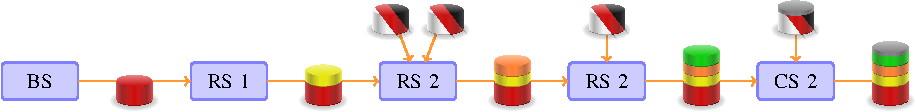
\includegraphics[width=\linewidth]{img/chain_c3}%
  \end{minipage}
  \quad%
  \begin{minipage}{.15\linewidth}
  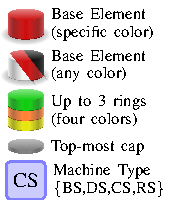
\includegraphics[width=\linewidth]{img/legend}%
  \end{minipage}
  \caption[Production chain of a high complexity
    product in the RCLL]{Production chain of a high complexity
    product in the RCLL~\cite{chapter-cps}}
  \vspace{-2mm}
  \label{fig:prod-chain}
\end{figure}
The \emph{RoboCup Logistics League (RCLL)}\footnote{RoboCup Logistics
  League website: \url{http://www.robocup-logistics.org}} is an
industry-oriented competition~\cite{LLSF-Rules-2016}. It tackles the
problem of production logistics in a smart factory, where mobile
robots have to plan, execute, and optimize the material and product
flow between machines to produce and deliver products according to
dynamic orders. Each competing team deploys a group of three robots
that has to build ordered products autonomously by interacting with
\emph{Modular Production Machines (MPS)} and transporting workpieces
between these machines.
\begin{wrapfigure}{r}{0.3\textwidth}
  \centering
  \vspace{-2.7ex}
  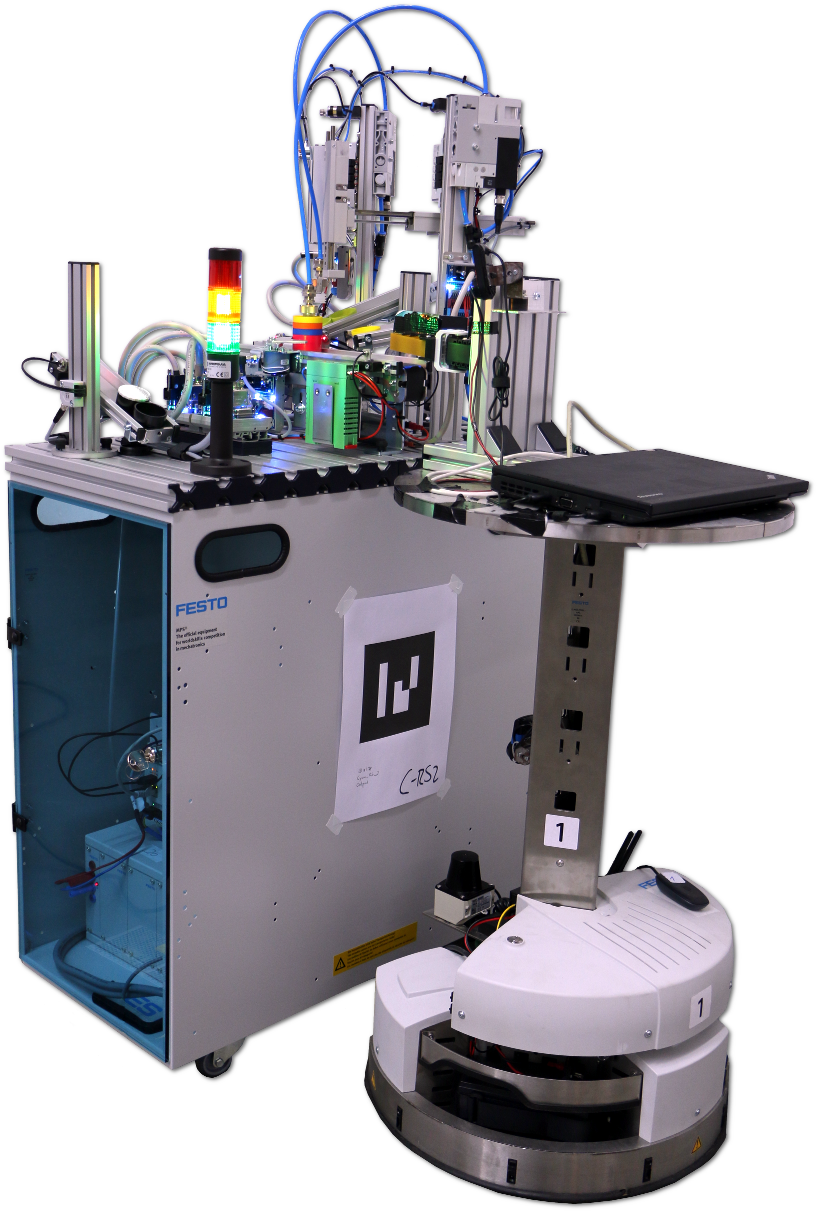
\includegraphics[width=0.3\textwidth]{img/rcll}
  \vspace{-4ex}
  \caption[Robot and MPS used in the RCLL]{Robot and MPS used in the RCLL~\cite{chapter-cps}}
  \label{fig:rcll-bot-mps}
\end{wrapfigure}
\reffig{fig:rcll-bot-mps} shows an RCLL robot filling a machine that mounts
colored rings on workpieces. The robots are based on the Festo
Robotino 3 platform, which uses a holonomic drive, and can be extended
and programmed by the teams. The robot shown in \reffig{fig:rcll-bot-mps} was
built by the Carologistics team and uses a laser range finder for
localization, a custom made gripper for handling workpieces, and
several cameras for detection of markers and light-signals mounted on
the machines~\cite{Carologistics2015,chapter-cps}. The game is
controlled by a software component called \emph{referee box (refbox)}
which acts as agent to control the environment~\cite{RCLL-Planning}.
It randomizes machine placements in the factory and
production orders, communicates with participating robots, controls
machines, and awards points.

The game consists of two phases. In the first phase, the
\emph{exploration phase}, the robots have to roam the factory to find
randomly placed machines, which are to be used later. By detecting the
light signal shown by the machines, the robots can determine the
machine-type. For correct reports of discovered machines to the refbox
the team is awarded with points, for incorrect ones points are subtracted.

In the second phase, the \emph{production phase}, the refbox announces
orders, which products have to be produced by the robots. Products
are build from colored cups with optionally mounted rings and a
colored cap.  \reffig{fig:prod-chain} shows the production chain for
building a high complexity product.  There are four different machine
types. The \emph{base-station (BS)} provides new bases, the colored
cups, as raw resource. The \emph{ring stations (RS)} mounts colored
rings on a workpiece after preparing it with a varying amount of
bases.  The \emph{cap-station (CS)} mounts black or gray caps to
finish a product after loading it with a cap form a shelf first.
Finally, the \emph{delivery-station (DS)} is used to deliver products.

A major challenge of the RCLL lies in the fully autonomous task
planning and coordination of the multi-robot system in the dynamic
environment with spatial information and time constraints. The
dynamism of the environment is caused by the randomization of the factory
layout, machine out-of-order times, product orders and
unknown obstacles, such as the robots of other teams. Furthermore,
baseline robotic challenges such as collision avoidance, perception
and behavior execution need to be solved. To outperform opponent
teams, the robots have to build as many ordered products as possible
and deliver them in the given time window. To cope with these
challenges, a decision making process needs the knowledge about the
environment, which is collected by the whole robot team. Therefore the
world model containing this knowledge has to be shared between the robots.
This can be done by the robot memory, which also allows
combining a global task planner looking in the future and a reasoner
for executing plans step by step and updating the world model with
current observations.

In the course of this thesis, we use a simulation of the
RCLL\footnote{\url{https://www.fawkesrobotics.org/projects/rcll-sim/}}
in the development and evaluation of the robot memory. The simulation
is based on the open source simulator Gazebo and models the RCLL with
multiple robots in a 3D environment with physics and
visuals~\cite{Gazebo-Design,Gazsim-Thesis,LLSF-Sim}. The simulation
was developed for multi-robot coordination evaluation and has
been proven as a useful tool for rapid testing and integration during
the development of robot software, e.g., for agent reasoning, robot
behavior, navigation graph creation, and collision avoidance. The simulation is
the primary testing and development environment for implementing the
robot memory in the RCLL because a full RCLL field is not available for us and
maintaining a team of robots with hardware and software takes much
effort and time. For the majority of robot software components, the
simulation is close enough to reality to yield similar results and
behaviors, because the only difference is the exchange of sensor data
and actuation software by simulated data and actuation. Exceptions are
visual perception by shape, and physical gripper actuation. Here, the
simulation uses an approach called \emph{multi-level abstraction},
which allows to simulate vision not only on the sensor data level
(providing a simulated image), but also on the perception level
(providing simulated perception results)~\cite{Multi-Level-Abstraction}.

\subsection{RoboCup@Home League}
The RoboCup@Home league is a competition about domestic service
robots~\cite{wisspeintner2009robocup}. Robots have to assist
humans in a variety of everyday tasks. These tasks include
serving
\begin{wrapfigure}{r}{0.2\textwidth}
  \centering
  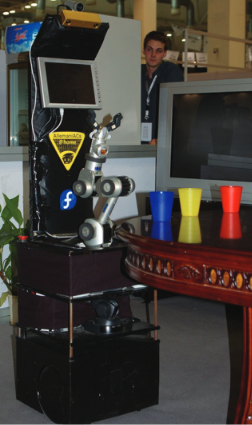
\includegraphics[width=0.2\textwidth]{img/ceasar}%
  \caption[RoboCup@Home robot Caesar tidying up]{RoboCup@Home robot Caesar tidying up~\cite{wisspeintner2009robocup}}
  \vspace{-3mm}
  \label{fig:athome}
\end{wrapfigure}
drinks, cleaning, setting tables, guiding or following people,
helping in emergency situations, shopping, and cooking.
\reffig{fig:athome} shows an @Home robot in the
competition.
%
The goal of the RoboCup@Home league is to foster and benchmark
research in the area of domestic service robots, to build a research
community and to envision autonomous multi-purpose robots helping
humans and especially elder people in the personal life.

The competition consists of multiple sub-tasks,
such as finding and manipulating objects, navigation tasks,
remembering persons, wait on tables, acting as
nurse, and an open challenge~\cite{athome-rules}.
To solve these tasks, robots need to
have a wide variety of abilities, including navigation, object
detection and manipulation, speech recognition, and especially human
robot interaction, which requires, for example, applying everyday
knowledge to incomplete task descriptions given by humans.

Important challenges in the @Home league are acting robustly in a
dynamic and only partial observable domestic environment and hybrid
reasoning with symbolic and spatio-temporal information.  The robot
memory can help here because it allows to collect information about
the concrete domestic environment and, for example, log object
observations to learn their distribution~\cite{deebul}.  Furthermore,
it can help with hybrid reasoning by transforming spatio-temporal
knowledge into symbolic knowledge with computables.  Another challenge
is that detecting and manipulating objects in a personal environment
can be difficult because the space the robot acts in, for example the
fridge, can be very clouded. The robot memory can help here, because
it is useful to keep an internal model of the environment instead of
only relying on the current perception results.

\section{Robot Software Frameworks}
\label{sec:robot-software-frameworks}
A \emph{robot software framework} can be defined as design and
implementation providing a possible solution for controlling a robot
with basic software libraries, a communication middleware, and a
run-time environment~\cite{tnthesis,orocos}.
%
Furthermore, it defines a standard for component interfaces that
allows building on a variety of open source solutions for robotic
problems. In the following, we introduce the widely used Robot
Operating System and Fawkes~\cite{Gazsim-Thesis}, which is used in
this thesis.
\subsection{Robot Operating System (ROS)}
\label{sec:ros}
The open source robot software framework
\emph{ROS}\footnote{\url{http://www.ros.org}} is a widely used
collection of useful open source libraries and tools for the
development process of robot software. It can operate on many robot
platforms from different domains and provides a standardized
integration framework~\cite{Ros,ros-book}. The components integrated
in ROS consists of processes called \emph{nodes}. These nodes can
exchange information over a peer-to-peer communication network. There
are communication channels called \emph{topics}. Nodes can register a
publisher to send messages on a topic or a subscriber to receive
messages sent over a specified topic. There are message types defining 
the fixed structure of a message with nesting. A central process
called \texttt{Roscore} manages the registration of publishers and
subscribers. It is also a broker for nodes and configurations.

In the RCLL, ROS is used by multiple teams~\cite{rc-2014}. The
Carologistics team uses ROS primarily for and localization and
visualization of sensor and perception data with the \texttt{Rviz}
package. In the years 2012 and 2013, Carologistics used the ROS package
\texttt{move\_base}, which provides local motion planning with
collision avoidance.

\subsection{Fawkes}
\label{sec:fawkes}
The basis for the thesis is the robot software framework
\emph{Fawkes}\footnote{\url{http://www.fawkesrobotics.org}}, which is
available as open source and developed at the Knowledge-based Systems
Group\footnote{\url{http://www.kbsg.rwth-aachen.de}} (KBSG) at RWTH
Aachen University~\cite{FawkesDesign,Fawkes-RCLL-2014}.  It is
designed to work with various robots in different domains and follows
a component-based software design, which separates functional entities
into individual software modules~\cite{component}. This enables
reusing software solutions for robotic problems, such as localization,
perception, reasoning, and behavior execution. Compiled components can
be loaded as \emph{plugins} at run-time.
%
Plugin activity is organized in threads to make use of multiple CPU
cores. The threads can be run concurrently or hooked into the
main-loop of Fawkes to order the execution into a
sense-think-act cycle.  This ensures that higher-level
components can use the latest perception data.  Fawkes softly
guarantees loop times by monitoring which threads are running for too
long and suspending to waking them up until they recovered. These are advantages in comparison to ROS,
because the components can be closer integrated. Features in Fawkes
are provided as \emph{aspects}. These are based on aspect-oriented
programming~\cite{aspect_oriented} and give access to particular
features. Threads that need to use a feature can inherit from the
corresponding aspect. For example, there are aspects for logging,
transforms, and specific external libraries~\cite{tnthesis}.

The communication between plugins uses a \emph{hybrid blackboard messaging}
paradigm. The blackboard lists structured entries called
\emph{interfaces}, which contain qualitative and quantitative
information.  Interfaces can be provided by at most one plugin at a time, the
writer, and read by other plugins, the readers. This allows a flexible
communication because the interface is independent from the concrete
writer and readers.  For example, sensor and actor plugins can be
exchanged by simulation plugins~\cite{Gazsim-Thesis,LLSF-Sim}.
Furthermore, the blackboard architecture simplifies
debugging because the current communication between two plugins,
determined by the state of the interface, can be viewed at
run-time. To send commands to an interface writer, for example a motor
command to the motor controller, readers can send messages to the
interface.
As a communication infrastructure between different components, the
blackboard only has limited possibilities to realize a robot memory.
Indeed the blackboard works well for providing some information and sending
commands. However the size
and structure of blackboard interfaces is fixed, and thus does not
allow to dynamically represent more or other information.  Furthermore
the blackboard does not support long-time memory, expressive querying,
or event-triggers.

\section{Planners and Reasoners}
\label{sec:planners}
In this thesis, there three planning and reasoning systems benefiting
from the robot memory. These are \emph{CLIPS}, a
rule-based production system, the \emph{Planning Domain Definition
  Language (PDDL)}, which incorporates a family of planning formalisms
into a standard programming language, and OpenRAVE, a \emph{motion
  planner} finding collision free actuation plans.  These systems are
representatives for often used types of planners and
reasoners. However, the robot memory is not limited to these because
it provides a general C++ interface, which can be used to integrate it
into more knowledge-based systems. The three systems presented here use the robot memory
to achieve new or improved functionality and are used for evaluation in this
thesis.

\subsection{CLIPS Rules Engine}
The CLIPS Rules Engine\footnote{\url{http://www.clipsrules.net/}} belongs to the class of \emph{rule-based
  production systems}, which can be defined as knowledge-based system
using forward chaining based on the \emph{Rete
  algorithm}~\cite{aimodern}. The Rete algorithm efficiently determines
which conditions of forward chaining rules can be matched by the
knowledge base, even with a large number of rules and facts by
constructing a data-flow graph and keeping partial
matches~\cite{Rete}. CLIPS is the basis of the currently used reasoner
by the Carologistics team in the RCLL and implements the high-level
game agent. The basic building blocks of the CLIPS Rules Engine are a
\emph{fact-base}, which is a working memory with small pieces of
information, a \emph{knowledge base} with rules and procedures, and an
\emph{inference engine} working with the knowledge base on the
fact-base~\cite{CLIPS-RM}. The pieces of information in the fact-base
are called \emph{facts} and consist of a name and a key-value
structure defined in a template for \emph{unordered facts},
e.g., \texttt{(position~(name~robot1)~(translation~2.5~1.0~0.0)}, or an
ordered list of values for \emph{ordered facts}.
\begin{figure}
\begin{lstlisting}[showlines,style=ReallySmallCLIPS, caption={CLIPS
    rule to change a robots state when the object it searched for is visible.},
  label=lst:clips-rule,
  emph={skill, args, state, target, res},
  emphstyle=\bfseries\color{green!80!black},
  emph={[2]\?skill, \$\?args, wait-for-lock, \?target, use,
  WAIT-FOR-LOCK, SKILL-EXECUTION, running},
  emphstyle={[2]\bfseries\color{blue!80!black}},
  morekeywords={retract, assert, modify, skill-call, skill-to-execute,
  wait-for-lock}]
(defrule found-machine
  ?s <- (state SEARCHING_FOR ?machine)
  (visible  (name ?machine))
  (position (name robot1) (translation $?pos))
  =>  
  (retract ?s) 
  (assert (state IDLE))
  (printout t "Found machine " ?machine " at " ?pos crlf)
)
\end{lstlisting} %$ This is just to fix Emacs highlighting due to dollar sign in code above
\end{figure}
An example rule is shown in \reflst{lst:clips-rule}. Rules are
composed of an \emph{antecedent} (lines 2-4) and a \emph{consequent} (lines 6-8). The
antecedent is the first part of the rule and describes the conditions
that have to be satisfied before the rule is considered for activation.
It consists of a list of patterns that have to be matched by facts in
the fact-base. For the antecedent in \reflst{lst:clips-rule}, there
have to be fitting \texttt{state}, \texttt{visible}, and
\texttt{position} facts with matching constants and variables, which
start with question marks. The consequent defines the procedure to execute when the rule is
activated. It usually modifies the fact-base by retracting and
asserting facts, for example to exchange the \texttt{state} fact. The
inference engine checks which rule antecedents are satisfied and puts
only them on the \emph{agenda}. Which rule of the agenda is executed,
is determined by a conflict resolution strategy such as highest
priority or earliest on the agenda. The consequent of the chosen rule
is executed and the inference engine checks again. \emph{Functions}
encode procedural knowledge, can have side effects, and can also be
implemented in C++.

The Carologistics RCLL agent implemented in CLIPS represents its
knowledge about the world, the \emph{world model}, in its
fact-base. It chooses actions to take by using a technique called
\emph{Incremental Reasoning}~\cite{CLIPS-Agent}: Whenever the robot is
idle, it searches for the next best task and executes it.  For each
task there is a rule with its preconditions in the antecedent and the
actions to take in the consequent. There are also rules for modifying
the world model, for example after finishing actions or getting new sensor
data, task execution, and coordination with other robots.  The
coordination of the robot team includes synchronizing their world
model and resource allocation. Because of the synchronization, each
robot knows what other robots noticed and changed in the
environment. The resource allocation ensures that no two robots try to
use the same machine at the same time or try to achieve the same goal by
choosing a redundant task. This coordination was already implemented
in CLIPS rules using Google Protocol Buffers (Protobuf)
messages. During this thesis, we developed an alternative
implementation based on the distributed robot memory that contains the
world model in a distributed database. On the one hand, this provides
an easy possibility to access the world model outside of CLIPS. On the
other hand, this is advantageous
because the database already provides efficient synchronization and
separating the synchronization from CLIPS decreases the
agent's complexity.

\subsection{Planning Domain Definition Language (PDDL)}
PDDL is a standardized language for planning
problems~\cite{PDDL}. It allows modeling the nature and behavior of a
domain as well as the \emph{actions} possible to perform in a
\emph{domain description}. An additional \emph{problem description}
defines the problem to solve. Both together can be given to a PDDL-based
planner that typically searches for a totally or partially ordered
sequence of actions, the \emph{plan}, to solve the problem.
\begin{figure}
\begin{lstlisting}[showlines,style=ReallySmallCLIPS, caption={PDDL
      action to pick up an object from a table},
  label=lsf:pddl-action,
  emph={skill, args, state, target, res},
  emphstyle=\bfseries\color{green!80!black},
  emph={[2]\?skill, \$\?args, wait-for-lock, \?target, use,
  WAIT-FOR-LOCK, SKILL-EXECUTION, running},
  emphstyle={[2]\bfseries\color{blue!80!black}},
  morekeywords={action, parameters, precondition, effect}]
(:action pickup
  :parameters (?ob)
  :precondition (and (on-table ?ob) (arm-empty))
  :effect (and (holding ?ob) (not (on-table ?ob)) (not (arm-empty)))
)
\end{lstlisting}
\end{figure}
\reflst{lsf:pddl-action} shows an example action contained in a domain
description.  Actions can have parameters and consist of preconditions
and effects. The precondition is a function free FOL sentence. In the
case of the picking action, it represents that the object that
should be picked is on the table and that the arm is empty. The effect
is a universally quantified and conditional FOL sentence, but not all FOL
sentences are allowed, for example sentences containing disjunctions~\cite{PDDL}. In the
example, the effect of the action is that the arm is not empty and the
object is now hold and not on the table any more. PDDL predicates,
such as \texttt{(arm-empty)} and \texttt{(on-table ?ob)} in the example,
describe properties and can be true or false.

There are various versions and extensions of PDDL which introduce new
concepts and features. For example, PDDL~2.1~\cite{PDDL2.1} adds
numeric values and continuous actions. This allows finding plans in
continuous environments where, for example, distances and travel times
matter. Planners based on PDDL can have the advantage of being able to find complete and
optimal or efficient plans depending on the model. However, this comes
with the drawbacks of high computational effort for larger domains and
the problem of adapting to events during plan execution. For example
when the domain is not fully observable, the robot could sense changes
in the environment or fail executing an action. This would require
notifying the planner, incorporating the changes in PDDL and
re-planning. To solve this problem, the robot memory allows
combining a PDDL-based planner with an execution in CLIPS. Then the
planner can generates an
efficient and complete plan with coarse actions and the executive can
carry out the plan step by step, while monitoring the execution and updating
the world model according to perceived changes. This world model is
written into the robot memory so that the world model with all changes
applied can be represented in PDDL.

Because PDDL is only a standardized language for formulating planning
problems, a concrete PDDL-based planner program is necessary to find plans. There
is a variety of planners. Many compete in the International
Planning Competition (IPC), which provides a benchmark and ranking for
multiple problem domains with different
complexities~\cite{planning-competition}. In this thesis, we use FF, a successful
planner of the IPC. FF uses
forward state space search and a heuristic that ignores the negative
literals in action effects~\cite{hoffmannFF}.

\subsection{Motion Planners}
Another kind of widely used planning in robotics is geometric motion
planning. It finds collision free trajectories in an n-dimensional
space to reach a goal position from the initial position. Common use cases
are planning the motion of a robotic arm to grasp or place something
and finding paths for driving robots. Thus motion planners use geometric
knowledge in contrast to logical reasoners and planners focusing on
symbolic knowledge.  When searching for an trajectory, it needs to take the degrees of
freedom, e.g., the joints of the robot or the maneuverability of the
robot base, into account and avoiding collisions with objects in the
environment. An example motion planner framework is \emph{MoveIt!},
which is available for ROS~\cite{MoveIt}. Another motion planner
framework already integrated into Fawkes is the \emph{Open Robotics
  and Animation Virtual Environment
  (OpenRAVE)}\footnote{\url{http://openrave.org/}}~\cite{OpenRave}. OpenRAVE
focuses on high-level commands as input and already integrates the
motion planning, visualization, and simulation. Thus it is a
convenient choice for a motion planner in Fawkes.

Motion planners can benefit from using a robot memory by accessing and
sharing information about objects and obstacles in the environment.
They can better work together with other planners and task execution
components because they can access the same knowledge base. This
avoids double state estimations, which can cause inconsistencies. To
be usable by motion planners, the robot memory has to be able to
represent hybrid information in the form of continuous positions and
time related events.

